\chapter{Twitter观点检索}
\label{OR}

\section{引言}

Twitter是一种流行的社交媒体,拥有超过5亿的用户并且每天产生多于3.4亿个tweet\footnote{\url{http://www.mediabistro.com/alltwitter/500-million-registered-users_b18842}}。人们喜欢在Twitter中分享消息并对人物、政治、商品、公司、事件等进行评论,使得Twitter变成一个拥有丰富观点信息的资源,不仅可以帮助人们做出决策,还可以辅助政府与公司收集有价值的反馈信息。例如,Jansen等人利用tweet作为某些商品的口碑信息进行分析\upcite{jansen2009twitter}; O'Connor等人分析了tweet的文本情感因素,以此作为公共的舆情分析\upcite{o2010tweets};Bollen等人利用Twitter中人们通过文本反映的情绪变化来预测股票市场\upcite{bollen2011twitter}。但是大多数已有的工作都是在tweet话题已经明确(涉及特定话题)的基础上的相关观点进行分析,并没有在给定某些人、商品或事件时,如何在Twitter中找到相关评论的工作。

本章中我们将讨论如何在Twitter中进行观点检索的工作,相对于上一章的Twitter信息检索工作,相关的观点tweet需要满足如下两个标准:
  \begin{enumerate}
  \item 与查询词话题相关。
  \item tweet包含涉及查询词的主观化观点,但不考虑观点的态度是正面的还是负面的。
  \end{enumerate}  
以下是两个关于查询词“UK strike”的tweet:
  \begin{description}
\item{a)} \emph{``Perhaps if the public sector workers on \#strike today go Christmas shopping then at least it will give the high street / UK economy a boost!"}
\item{b)} \emph{``UK: BBC - Up to TWO Million Set to Strike http://t.co/wBrsgrKh \#tcot \#gop \#ows"}
  \end{description}  
这两个tweet中,Tweet(a)是与查询词相关的观点tweet(本章以后我们简称为相关tweet);Tweet(b)不是与查询词相关的tweet,因为它没有作者对于话题“UK strike”的观点。

博客和Web网页中的观点检索已经被大量的研究\upcite{zhang2007opinion,he2008effective,zhang2008generation,gerani2010proximity,gerani2012aggregation}。最近文本检索会议(Text Retrieval Conference-TREC)也组织了对于博客的观点检索评测(博客 Track)\upcite{ounis2006overview,macdonald2007overview,ounis2008overview,macdonald2010blog}。传统的观点检索面对的主要问题是:(1)文档的观点性判定;(2)文档的观点是否是对给定话题的评价。除了以上普遍存在的问题,Twitter中的观点检索难度更大,主要原因是:

\begin{enumerate}
\item{\textbf{文本简短}}:tweet文本十分简短且最多只有140个字符。这种短文本属性造成人们经常使用缩写词或短语等压缩tweet的文本长度\upcite{gouws2011contextual},Luo等人也发现如果tweet中存在很多链接、hashtag、固定字符串(例如,“@username”和“RT @username”),也会造成人们经常使用缩写词或短语\upcite{luo2012improving},这样tweet中就会大量存在未登录词,结果造成许多词无法识别,使得查询词与tweet中的文本无法在检索时进行很好的词匹配\upcite{metzler2011usc}。
\item{\textbf{文本质量差异大}}:对于观点检索来说,Twitter是一个全新的领域,存在大量的垃圾信息和文本变化大的tweet,但是大多数网页(如新闻网页)都是一些文本质量相对较高的正式文档,而tweet大多数是个人发布的非正式文本。这就造成tweet的文本质量明显不同于其他文本,对于观点检索来说是个巨大的挑战。
\end{enumerate}

但是Twitter自身的特点可以帮助Twitter中的观点检索。因为Twitter中包含丰富的社交媒体特征,例如,以前发布过多少tweet的用户信息。这些特征可以弥补词方面检索不匹配的缺点,间接提高观点检索的效果。另外,一些人们发布tweet的习惯使得tweet可以被看成一个结构化文本,这种结构化信息也可以帮助Twitter中的观点检索。

例如,人们经常在字符串“RT @usename”前面加评论信息,这种类型的tweet一般都是主观化的tweet。而大多数新闻媒体用户(例如,BBC News)发布的tweet一般都是给出一段介绍文本,紧接着给出一个相关链接,直观上这种类型的tweet一般是客观的信息。更重要的是,这些结构化信息不依赖于特定话题。因此这就促成我们利用这些社交媒体特征与tweet的结构化信息帮助Twitter的观点检索。

本章中我们将介绍如何利用机器学习构造检索模型的方法实现Twitter中的观点检索,这种方法利用了社交媒体特征,观点化特征和话题相关特征(例如,Okapi BM25\upcite{robertson1995okapi,robertson1996okapi}和向量空间模型\upcite{salton1975vector})。实验结果表明当检索模型考虑tweet中是否存在链接、提及、作者曾发布过多少tweet、粉丝数目和观点化特征时,Twitter中的观点检索效果明显提高。

另外,我们利用基于语料的方法构造观点化词典评价tweet中文本的观点化程度,但是这种方法依赖手工标注的语料,手工标注语料耗费人力与时间,而且对tweet的观点化评价是一个与话题相关的问题\upcite{jiang2011target,liu2012emoticon,meng2012entity},在对tweet进行观点化评价中不可能针对每个话题手工标注语料进行词典构造,为此我们提出了一种新的方法来解决以上问题。这种方法利用社交媒体特征与tweet文本的结构化特征自动收集一些近似主观化tweet(`pseudo' subjective tweet-PST)和近似客观化tweet( `pseudo' objective tweet-POT),收集好的这两种数据集合能够自动生成观点化词典来评价tweet的观点化程度。我们将这种方法与传统的手工标注语料进行了实验比较,发现在Twitter观点检索中,该方法取得的效果与手工方法效果相当,当自动收集与话题相关的近似主观化tweet和近似客观化tweet时,Twitter观点检索效果获得进一步提高。

本章的主要工作如下:
\begin{enumerate}
\item 根据我们的调研这是第一次对Twitter进行观点检索的研究。我们发布了研究过程中所使用的检索数据\footnote{下载地址:\url{https://sourceforge.net/projects/ortwitter/}},这个数据包括50个查询词和其对应的5000个手工标注相关与不相关的tweet。
\item 我们提出了一种Twitter观点检索方法,这种方法利用社交媒体特征与tweet观点化特征,并在实验结果上显著优于优化的BM25基准系统和VSM系统(分别提高56.82\%和33.75\%)。
\item 另外,我们还提出了一种基于社交媒体特征与tweet文本结构化信息收集近似主观化tweet(`pseudo' subjective tweet-PST)和近似客观化tweet( `pseudo' objective tweet-POT)构造主观化词典的方法,并以此评价tweet的观点化程度,实验结果表明这种方法对于tweet的主观化评价能够取代传统手工标注语料构造词典的方法,并在Twitter观点检索中取得效果相当的结果,当考虑针对话题收集PST和POT时,使用该方法的Twitter观点检索效果更好。
\item 最后我们重新标注了TREC Tweets2011数据\upcite{ounis2011overview},使其能够对Twitter观点检索方法能够进行评价,实验结果进一步验证了我们方法的有效性。
\end{enumerate}

\section{相关工作}
我们从两个方面讨论相关工作:Twitter中的观点挖掘和TREC观点检索。Twitter中的观点挖掘主要是通过自然语言处理技术在Twitter中发现和跟踪人们对事件、产品等的观点和态度;TREC观点检索是在博客数据集合中,给定查询词,找到与查询词话题相关且带观点的博客文档。前者能够帮助我们在观点检索任务中对tweet进行观点判定,后者可以为我们在Twitter中进行观点检索提供技术思路。

\subsection{Twitter观点挖掘}
Twitter吸引了成千上万的用户在这个平台上发布各种观点,这也使得其成为一个研究的热点对象。

Jansen等人研究了关于特定品牌的tweet\upcite{jansen2009twitter},他们设计了一个舆论感知器,量化品牌的公司与消费者之间的紧密关系,他们发现19\%的tweet包含或提及与商品有关的信息,这其中大约20\%包含人们对商品的观点。这说明Twitter可以成为公司收集消费者对于商品文本评价的资源库。

O'Connor等人通过分析tweet的态度度量了社会舆情\upcite{o2010tweets},这种方法可以替代传统的问卷调查。他们分析了消费者对于商品态度的tweet和对美国总统施政评价的tweet,结论是这种简单的方法可以替代费用高昂且实时性要求强的社会问卷调查方式。

Bollen等人从大规模Twitter数据中分析了道琼斯工业平均指数(Dow Jones Industrial Average\footnote{\url{http://en.wikipedia.org/wiki/Dow_Jones_Industrial_Average}})与tweet的情绪倾向性存在很强的联系\upcite{bollen2011twitter}。他们发现公众的情绪状态的变化的确可以在大规模Twitter数据中被跟踪,这种不断变化的信息,可以成功地帮助预测股市。这表明Twitter是一个收集公众意见的重要来源。

以上的研究主要集中在给定话题的情况下挖掘公众的观点,而不是如何在Twitter中找到特定话题的观点tweet。我们本章考虑的问题是在给定查询词的情况下,在Twitter中检索相关观点。

另外的相关工作是Twitter的情感倾向性分析,主要分析观点tweet是正面的肯定态度,还是负面的否定态度。Davidov等人利用机器学习的方法对给定tweet进行情感倾向性判定\upcite{davidov2010enhanced},他们利用hashtag和表情符号自动构造了大量的训练样本,以此提高分类效果。Barbosa和Feng从网站\emph{Twendz}\footnote{\url{http://twendz.waggeneredstrom.com/}}, \emph{Twitter Sentiment}\footnote{\url{http://twittersentiment.appspot.com/}} 和\emph{TweetFeel}\footnote{\url{http://www.Tweetfeel.com/}}中收集大量的训练数据进行情感倾向性判定\upcite{barbosa2010robust},Jiang等人通过结合话题相关的特征和tweet所在上下文信息,改善了话题相关的tweet的情感倾向性分析\upcite{jiang2011target}。其他还有大量的相关工作从不同的角度分析和提高tweet情感倾向性分析的效果\upcite{kouloumpis2011twitter,agarwal2011sentiment,tan2011user,wang2011topic,brody2011cooooooooooooooollllllllllllll,hu2013exploiting,mukherjee2012twisent,saif2011semantic,marchetti2012learning,aisopos2012content,martinez1sentiment,kontopoulos2013ontology,hu2013unsupervised,bollen2011modeling,thelwall2011sentiment,bermingham2010classifying,paltoglou2012twitter,chung2011can,conover2011political,gonzalez2011identifying}。

情感分析的目的是识别文本态度的倾向性,我们的工作考虑的是如何在Twitter中找到观点性的tweet,不论观点是正面的还是负面的。

\subsection{TREC观点检索}
博客数据中的观点检索第一次在TREC 2006中组织评测,然后TREC2007与TREC2008也分别进行了相同任务的评测\upcite{ounis2006overview,macdonald2007overview,macdonald2007overview}。大多数参与评测的机构都采用两阶段的方法,首先在数据中检索到与查询词话题相关的文档集合,然后对文档集合中的文档根据各种不同的观点化度量方法进行文档的重排序,以此获得相关文档。

另外还有一些观点检索的工作。Eguchi和Lavrenko第一次提出了观点检索的问题\upcite{eguchi2006sentiment},他们结合了话题相关模型与情感倾向性相关模型,以此组合成一个整体模型对文档进行排序,这种方法的有效性在MPQA语料中得到验证。Zhang和Ye,Huang和Croft也提出了他们自己的整合话题相关与情感倾向性相关的模型,以此检索观点\upcite{zhang2008generation,huang2009unified}。Gerani等人第一次将排序学习的方法引入观点检索中\upcite{gerani2009investigating}。进一步的工作还从不同的角度进行相关研究\upcite{mishne2006multiple,na2009improving,gerani2010proximity,santos2009integrating,zhang2008improve,vechtomova2010facet,vechtomova2007using,gerani2009investigating,bermingham2009study,jia2009effect,li2010unified,lee2010high,gerani2011aggregating,he2009fitting,amati2010performance,seki2009adaptive,orimaye2011sentence,guo2012exploiting,xu2012find,orimaye2012can}。以上所有的工作针对的数据不是博客就是Web网页,我们考虑的问题是Twitter中的观点检索,这种新的社交媒体存在大量的社交媒体特征,需要将此考虑到检索模型当中。

观点检索任务的难点在于如何度量文档的观点化程度。He等人基于主观词的出现来评价文档的观点化程度\upcite{he2008effective}。这些主观词自动地由标注语料产生,他们将观点化的相关文档视为主观文档,话题相关的文档视为客观文档,然后词的主观化程度可以通过度量词在两个文档集合中的分布差异性进行度量。Amati等人采用类似的方法自动构造观点词来帮助检索\upcite{amati2008automatic}。Seki和Uehara利用结合邻近词依赖关系的统计语言模型来度量文档的观点化程度进行排序\upcite{seki2009adaptive}。Jijkoun等人提出了一种依赖语法规则自动标注数据,并以此自动构造话题相关主观词的方法\upcite{jijkoun2010generating}。Li等人提出了一种基于话题词与情感词配对评价文档观点化程度的观点检索方法\upcite{li2010unified}。以上所有的方法都依赖人们手工标注的语料构造情感词典。

不同于上面的方法,Zhang等人利用网站RateitAll.com的评论信息和其他网页作为近似主观句(`pseudo' subjective sentence-PSS)的资源,然后利用维基百科的页面作为近似客观句(`pseudo' objective sentence-POS)的资源\upcite{zhang2007opinion}。他们假设主观性句子应该在评论信息中占据主要部分,客观性句子可以被忽略,而维基百科的客观性句子占据比例恰好相反。接着他们利用近似主观句集合和近似客观句集合构造SVM句子主观性分类器,这个分类器可以对新句子进行观点化度量,最后他们利用这个观点化度量与句子话题相关程度综合对文档进行排序。本章中,我们采用类似的方法,利用社交媒体特征与tweet文本的结构化信息自动生成近似主观化tweet(`pseudo' subjective tweet-PST)和近似客观化tweet( `pseudo' objective tweet-POT),以此帮助Twitter中的观点检索。

\section{基于排序学习的Twitter观点检索框架}
为了构造一个能够帮助Twitter观点检索的模型,我们将研究社交媒体特征与tweet观点化特征对于这个任务的有效性。我们将设计一系列特征,并将其应用到排序学习模型的场景中(Learning to Rank)\upcite{liu2009learning}。

 \subsection{Twitter观点检索排序学习框架}
 正如~\ref{LTR}所介绍的,排序学习是一种将特征有效地整合到排序模型的机器学习算法。我们将一系列与Twitter观点检索相关的特征引入此框架,话题对应的tweet分别人工标记是否为相关tweet。我们使用RankSVM进行排序模型的学习\upcite{Joachims:1999:MLS:299094.299104}。

 \subsection{Twitter观点检索相关特征}
第一章介绍了本文主要的两个研究问题:(1)人们在Twitter中如何用自然语言描述话题和表达观点?(2)以Twitter为代表的社交媒体有何新特点?如何利用这些特点帮助获取信息?因此,我们从两个方面设计Twitter观点检索相关特征:
  \begin{enumerate}
\item{\textbf{社交媒体特征(Social Feature)}}:主要涉及一些Twitter特有的属性特征和与tweet作者有关的用户信息。
\item{\textbf{观点化特征(Opinionatedness Feature)}}:主要涉及如何评估tweet的观点化程度。
\end{enumerate}

社交媒体特征主要是想通过分析Twitter新媒体的特点,发现哪些社交媒体新特征与观点化的tweet存在关系,以此帮助Twitter观点检索。比如,用户的粉丝数目、认证用户等,是否会影响tweet的观点化偏置。Tweet的观点化评价(即观点化特征)是观点检索的重要部分,我们的目的是通过分析人们在Twitter中如何表达观点及其特定的文本表现形式,以此提出方法来帮助tweet观点化的判定,最终提高Twitter观点检索的效果。

下两节我们将详细介绍这些特征是如何设计并应用到Twitter观点检索当中的。

\section{社交媒体特征}

为了分析哪些Twitter新媒体特点与tweet观点化存在潜在的关系,我们从Twitte社交媒体特征的两个方面进行考虑:Twitter特定的属性和tweet的用户信息。

\subsection{Twitter特定特征}
人们在发布tweet时经常有一些习惯,这些习惯可能与tweet的观点化程度相关:

  \begin{enumerate}
\item{\textbf{链接(URL)}}:Twitter中分享链接是非常普遍的。大多数包含链接的tweet都是首先给出一个客观描述性的文本,然后紧接着给出一个与该文本相关的链接(例如,BBC News发布的tweet)。另外,Twitter中大多数的垃圾tweet都包含链接。因此,我们设计了链接特征,用来描述给定tweet中是否存在链接。如果tweet中存在链接,则该特征值为1,否则为0。
\item{\textbf{提及(Mention)}}:在一个tweet中,人们经常使用符合“@username”来提及某人或回复某人。这种类型的tweet往往都是一些个人消息。以前的研究发现个人消息比官方消息更有可能包含观点\upcite{gerani2011aggregating},所以我们用一个布尔特征来描述一个tweet中是否包含“@username”,并以此帮助Twitter中的观点检索。
\item\textbf{\textbf{主题词(Hashtag)}}:hashtag是由``\#" 符合与一个词组合而成,它主要用来表示tweet的主题。我们设计布尔特征来描述tweet中是否包含hashtag。
\item\textbf{\textbf{Tweet发布时间(Recency)}}:Twitter实时地产生大量的tweet流,直觉上如果发布的tweet离用户查询时间越接近,则越有可能是相关tweet,因此我们设计了tweet发布时间到用户输入查询词的时间差 (以秒计)的特征。
\end{enumerate}

\subsection{用户特征}
Twitter的用户和用户之间的关系是一个典型的社交网络,这些丰富的用户信息可以用来帮助Twitter的观点检索:

  \begin{enumerate}
  \item{\textbf{发布数目(Statuses)}}:Twitter用户以往发布tweet的多与少反映了用户的活跃程度。直觉上,如果一个用户发布大量的tweet,他很有可能是垃圾用户。因此我们设计了特征tweet的作者发布tweet数目帮助Twitter观点检索。
   \item{\textbf{粉丝数目和朋友数目(Followers and Friends)}}:在Twitter中用户可以关注任意数量他感兴趣的其他用户。如果{\em userA}关注 {\em userB},则 {\em userB}发布的所有tweet用户{\em userA}都能在自己的页面中自动显示。我们将{\em userA}称为粉丝(Follower),将{\em userB}称为朋友(Friend)。用户的粉丝数目决定了用户受欢迎的程度,例如,新闻媒体用户往往比普通用户拥有更多的粉丝。同样,用户的朋友数目也反映了用户的特点,例如,大多数垃圾用户的朋友数目都远远大于其粉丝的数目。我们设计了这两个特征帮助Twitter观点检索。
   \item{\textbf{分组数目(Listed)}}: 一个用户可以将其朋友按照一定的标准(例如,兴趣和社会关系)划分到几个组中。如果一个用户被分到多个组中,则说明很多人都对这个用户的tweet感兴趣。我们用一个特征来记录给定tweet的作者被分到不同组的数目,以此帮助Twitter观点检索。
  \end{enumerate}

\section{观点化特征}
\label{form}
对于观点检索任务来说,评估一个tweet的观点化程度显然是不可或缺的。以前对于评估文档观点化程度的方法大致可以分成两类\upcite{na2009improving}:
  \begin{enumerate}
  \item 基于机器学习的分类方法。
  \item 基于情感词典的方法。
   \end{enumerate}
   我们采用基于情感词典的方法,因为这种方法简单且不需要利用机器学习技术。但是,常用的情感词典,如MPQA Subjectivity Lexicon\footnote{下载地址:http://www.cs.pitt.edu/mpqa/}, 可能对于Twitter来说不适用,因为tweet的文本很短且非正式,存在大量的情感表达方式不出现在情感词典中。因此,我们利用语料来构造适应Twitter的情感词典。通过计算tweet中特定的词,帮助评估tweet文本的观点化程度。我们利用手工标注的主观tweet集合和客观tweet集合,计算词的chi-square分值,此分值可以评估词的观点化权重。chi-square分值是一种词对于主观tweet集合或客观tweet集合关联程度的度量方法。对于一个tweet,我们只保留那些chi-square分值不低于$m$ 的词。对于tweet~$d$的观点化程度,评价函数是:

$$Opinion_{avg}(d)=\sum_{t\in d, \chi^{2}(t)\geq m}p(t|d)\cdot Opinion(t)$$

其中$p(t|d)=c(t,d)/|d|$是词$t$ 在tweet $d$中的相对词频,$c(t,d)$是该词在tweet~$d$中的词频,$|d|$表示tweet~$d$所包含的词数。

$$Opinion(t)=sgn(\frac{O_{11}}{O_{1*}}-\frac{O_{21}}{O_{2*}})\cdot \chi^{2}(t)$$

这里,$sgn(*)$是一个符号函数,$\chi^{2}(t)$ 是计算词chi-square值的函数。

$$\chi^{2}(t)=\frac{(O_{11}O_{22}-O_{12}O_{21})^2\cdot O}{O_{1*}\cdot O_{2*}\cdot O_{*1}\cdot O_{*2}}$$ 

表~\ref{chi-square}中,$O_{ij}$是用来表示在主观tweet集合或客观tweet集合中存在多少条tweet包含词$t$或不包含词$t$,例如, $O_{12}$表示在主观tweet集合中不包含词$t$的tweet数目。

\begin{table}[htp]
\centering
\caption{pearson's chi-square表}
\label{chi-square}
\begin{tabular}{|c|c|c|c|}
\hline
 & t & $\neg{t}$& Row total\\
 \hline
 Sub. set & $O_{11}$ & $O_{12}$& $O_{1*}$\\
 \hline
Obj. set & $O_{21}$ & $O_{22}$& $O_{2*}$\\
 \hline
 Col. total & $O_{*1}$ & $O_{*2}$& $O$\\
 \hline
\end{tabular}
  \begin{tablenotes}
        \footnotesize
\item  $O_{1*}=O_{11}+O_{12}$;$O_{2*}=O_{21}+O_{22}$;$O_{*1}=O_{11}+O_{21}$;$O_{*2}=O_{12}+O_{22}$;$O=O_{11}+O_{12}+O_{21}+O_{22}$
\end{tablenotes}
\end{table}

大规模手工标注主观tweet和客观tweet非常耗时耗力,且tweet是否存在观点还与领域有关\upcite{jiang2011target,liu2012emoticon,meng2012entity}。例如,与话题“android”相关且存在观点的tweet可以用词“\emph{open}”、“\emph{fast}”、“\emph{excellent}”进行描述,但是这些词不可能是对某些特定事件的观点描述(例如,“UK strike”)。另外,我们也不可能对于每个话题人工标注大量的主观tweet和客观tweet。基于以上我们提出了一种自动收集近似主观化tweet(`pseudo' subjective tweet-PST)和近似客观化tweet( `pseudo' objective tweet-POT)的方法。

在Twitter中一些简单的tweet文本结构化信息和用户信息可以帮助自动收集大量的PST和POT。例如,人们经常在转发其他人发布的tweet前面加上自己的评论信息,这种结构的tweet大部分是主观化的tweet。另外,许多新闻媒体用户喜欢发布一段客观描述的文本加上链接的tweet,这些新闻媒体用户一般曾经发布过大量的tweet且粉丝众多。我们定义近似主观化tweet(`pseudo' subjective tweet-PST)和近似客观化tweet( `pseudo' objective tweet-POT)如下:

 \begin{enumerate}
\item{ \textbf{近似主观化tweet(`pseudo' subjective tweet-PST)}}:一种tweet,它在转发tweet的字符串“RT @username”前面存在其他文本。例如,tweet“\emph{I thought we were isolated and no one would want to  invest here! RT @BBCNews: Honda announces 500 new jobs in Swindon \url{bbc.in/vT12YY}}”是一个PST。
\item{\textbf{近似客观化tweet( `pseudo' objective tweet-POT)}} : 如果一个tweet满足如下条件:
\subitem{a:}包含链接;
\subitem{b:}tweet的作者曾经发布过大量的tweet且粉丝众多。

这种tweed称为POT。例如,tweet“\emph{\#NorthKorea:\#KimJongil died after suffering massive heart attack on train on Saturday, official news agency reports \url{bbc.in/vzPGY5}}”。
\end{enumerate}

利用上面的定义,我们可以简单地构造一些规则并从Twitter中收集大量的PST和POT。我们假设在收集的PST集合中,所有的tweet都是主观性的文本,而收集的POT集合中,所有的tweet都是客观性文本。虽然这并不是100\%准确,但是,PST集合中主观性的tweet必定占据绝大部分,使得客观性的tweet可以被忽略,而POT集合情况则恰好相反。另外,文本的结构化信息和用户信息与tweet的话题无关,因此如果能有大量话题关联的tweet,则可以从中收集大量话题相关的PST和POT。

\section{Twitter观点检索实验}
本章我们将上面讨论的特征对于Twitter观点检索的效果进行实验验证。

\subsection{Twitter观点检索实验数据}
据我们所知,目前还没有关于Twitter观点检索的评测数据。为了从Twitter中找到给定话题的话题相关tweet且其包含对此的观点,我们自己构造了Twitter观点检索数据。

我们在2011年11月利用Twitter API爬取了3000万个tweet,所有的tweet都是英文的\footnote{我们利用语言检测工具过滤非英语tweet,下载地址:\url{http://code.google.com/p/language-detection/}}。我们使用Lucene\footnote{下载地址:\url{http://lucene.apache.org}}对所有tweet建立索引并构造搜索引擎。7个用户使用了该搜索引擎,7人中包括6名男性和1名女性,所有的用户都不是母语为英语的人,但是他们的英语都有很好的基础。这些用户可以在搜索引擎中提交他们感兴趣的任意查询词,给定查询词,搜索引擎将根据BM25返回100个得分最高的tweet。我们使用Lucene-BM25\footnote{下载地址:\url{http://nlp.uned.es/~jperezi/Lucene-BM25/}} 计算每个tweet对于查询词的BM25分值。在计算BM25分数时,相关参数都使用默认设置($k_1=2$;$b=0.75$)。最后所有的查询词都是在2011年12月1日提交的。

根据tweet是否与查询词话题相关且包含观点的定义,提交查询词的用户对返回的tweet进行标注,如果tweet与查询词话题相关且包含观点,则这个tweet的类别分值标为1,否则标为0。我们在这里只考虑tweet是否包含观点,并不考虑观点的情感倾向性,另外,tweet仅仅话题相关或只包含话题无关的观点,我们都将其视为不相关tweet。


最终我们搜集了50个查询词和5000个标注数据,其中每个查询词对应100个tweet。我们将这50个查询词分成6个类别,表~\ref{OR_data}给出了这6个类别的查询词及其相关tweet数量。另外,所有查询词的平均长度为1.94个词,每个查询词平均相关tweet为16.62个。


我们进一步考虑了这些标注数据的可靠性。对于每一个查询词,我们随机选取了10个对应的tweet叫另外两个标注者进行相关标注。这两个标注者标注数据的kappa分数为0.54,这说明我们的Twitter观点检索数据具有“好”的可靠性。

\subsection{Twitter观点检索实验设置}
我们将验证上两节介绍的特征对于Twitter观点检索的作用。对于排序学习,我们使用了SVM Rank工具\footnote{下载地址:\url{http://www.cs.cornell.edu/people/tj/svm_light/svm_rank.html}}。在排序学习模型的训练与测试过程中,我们使用了线性核函数。另外,所有结果都是将模型参数调到最优。为了解决测试数据规模较小造成结果偏置的问题,我们使用了5次交叉验证的方法。每次折叠过程,我们都将数据分成训练数据、测试数据、验证数据,其中训练数据包含30个查询词,而测试数据和验证数据各包含10个查询词。对于评价指标,我们依然使用平均准确率(\emph{Mean Average Precision-MAP} ),因为这个评价指标在TREC的检索任务中被经常使用且具有很好的排序算法效果区分性与稳定性\upcite{Manning:2008:IIR:1394399}。

\begin{table}
\centering
\caption{Twitter观点检索查询词及其相关tweet数目}
\label{OR_data}
\begin{tabular*}{\textwidth}{@{\extracolsep{\fill}}|r rr|}
  \hline
\textbf{组织}		&	\textbf{产品}		&	\textbf{人物}		\\
 \hline
pixar,	23	&	Mac book pro,	37	&	Jennifer Aniston,	40	\\
manchester city,	21	&	iphone4s,	32	&	chris paul,	39	\\
htc,	19	&	kinect,	30	&	Obama,	35	\\
Syria,	17	&	itouch,	25	&	bill gates,	16	\\
iran,	15	&	kindle fire,	16	&	Maggie Q,	13	\\
Manchester United,	15	&	iOS5 Jailbreak,	12	&	owl city,	12	\\
disney,	12	&	galaxy note,	11	&	paul graham,	10	\\
Lenovo,	10	&	Xbox 360,	7	&	steve jobs,	9	\\
microsoft,	6	&	google venture,	7	&	Kai-Fu Lee,	1	\\
Calvin Klein,	5	&	new Google Bar,	5	&			\\
fossil,	5	&	EA Daily Deals,	0	&			\\
intel,	3	&	SIEMENS fridge freezer,	0	&			\\
channel,	0	&			&			\\
 \hline								
 \hline								
\textbf{其他}		&	\textbf{事件}		&	\textbf{电影、电视剧}		\\
 \hline
job hunting,	79	&	iran nuclear,	35	&	Breaking Dawn,	49	\\
speech recognition,	15	&	American Music Awards,	25	&	big bang,	41	\\
machine learning,	4	&	UK embassy,	21	&	Two And A Half Men,	35	\\
new start-ups,	2	&	UK strike,	7	&	inside job,	2	\\
immigrate to canada,	1	&	ARTIST OF THE YEAR,	7	&			\\
systems biology,	0	&			&			\\
text mining,	0	&			&			\\
 \hline
\end{tabular*}
\end{table}

\subsection{基准系统(Baseline)}
\label{Baseline}
目前据我们所知,Twitter中的观点检索还没有相关的工作,因此我们只能通过选择相近的工作(比如上一章的Twitter信息检索的方法)作为比较。但是由于我们的研究目的是分析哪些因素能够影响Twitter中观点检索的效果,因此在基准系统的选取上,我们选择了简单的基于话题相关的模型(如BM25)。一般地,与多个基准系统比较检索效果能够更好地验证检索方法的有效性,因此在我们的实验中,我们采用了两个基准系统:
  \begin{enumerate}
\item{\textbf{BM25}}:利用优化的Okapi BM25对tweet进行打分,然后排序。
\item{\textbf{VSM}}:利用向量空间模型(Vector Space  Model)对tweet与查询词进行话题相关性打分,然后排序\upcite{salton1975vector}。
\end{enumerate}

在信息检索的排序算法中,Okapi BM25是其中最著名的基于概率的评估查询词与文档内容相关性的算法。给定查询词$q$,$t$为查询词中的词,一个文档$d$的BM25分数为:

$$BM25(q,d)=\sum_{t\in q}log(\frac{N-df_i+0.5}{df_i+0.5}*\frac{(k_1+1)(tf_i)}{k_1((1-b)+b\frac{dl}{avdl})+tf_i})$$

其中$tf_i$表示词$t$的词频,$df_i$表示词的文档频率,$N$表示数据集合中的文档数量,$dl$是文档长度(词数),$avdl$是文档集合中所有文档的平均长度。两个参数$k_1$和$b$分别决定了词频和文档长度的归一化对于分数的影响。以下的实验中,我们将利用验证数据集对参数$k_1$和$b$进行优化,以此得到最优的基于Okapi BM25的Twitter观点检索排序算法。

因为tweet是典型短文本,而BM25算法对于文本长度的变化十分敏感,因此我们引入了另一种简单的信息检索排序算法VSM。VSM最早由Salton等人提出\upcite{salton1975vector}。VSM算法中,文档$d_j$和查询词$q$ 可以分别表示成两个$t$维的词向量$d_j= (w_{1,j},w_{2,j},...,,w_{t,j})$和$q= (w_{1,q},w_{2,q},...,,w_{t,q})$,其中$t$ 表示文档集合中不同词数目,每一维表示一个词,有许多方法可以决定词的权重$w$,我们使用经典的$tf$-$idf$ 度量词的权重:

$$w_{t,d}=tf_{t,d}*log(\frac{|D|}{|d'\in D|t\in d'|})$$

$tf_{t,d}$ 是词$t$在文档$d$中的词频,$log(\frac{|D|}{|d'\in D|t\in d'|})$ 是倒转文档频率, $|D|$是文档集合中文档数量,$|d'\in D|t\in d'|$文档集合中包含词 $t$的数量。文档$d_j$ 和查询词$q$的相似度可以通过计算两个向量的余弦夹角得出:
$$sim(d_j, q)=\frac{\sum_{i=1}^Nw_{i,j}*w_{i,q}}{\sqrt{\sum_{i=1}^Nw_{i,j}^2}*\sqrt{\sum_{i=1}^Nw_{i,q}^2}}$$
我们利用Lucene实现VSM的计算。

\subsection{Twitter观点检索实验结果及分析}
我们将实验分成以下几个方面进行讨论:

\begin{enumerate}
\item 社交媒体特征能否帮助Twitter中的观点检索?({见~\ref{SFE}})
\item 观点化特征能否帮助Twitter中的观点检索?({见~\ref{OFE}})
\item 基于话题相关的PST和POT能否比话题不相关的PST和POT更好地帮助Twitter中的观点检索?(见~\ref{TDPPFE})
\item  PST和POT能否帮助观点化tweet的识别?({见~\ref{STC}})
\item 那种Twitter观点检索模型达到最佳效果?({见~\ref{AFE}})
\end{enumerate}

另外,表~\ref{Features_Sum} 简要概述了Twitter观点检索所使用的相关特征。

\begin{table}
\centering
\caption{Twitter观点检索特征概况}
 \label{Features_Sum}
  \begin{tabular*}{\textwidth}{@{\extracolsep{\fill}}| l l p{1.7in}|}
\hline
\textbf{基准系统特征(Baseline Features)} & \textbf{取值范围}& \textbf{描述} \\
 \hline
BM25 & $(0,+\infty)$ &tweet的BM25分值\\
VSM  & $(0,+\infty)$ & tweet的VSM分值 \\
 \hline 
 \hline 
\textbf{社交媒体特征(Social Media Features)} & \textbf{取值范围} & \textbf{Description} \\
 \hline
 链接(URL)& $0$ or $1$ & tweet中是否包含链接 \\
 提及(Mentions)& $0$ or $1$ & tweet是否包含提及 \\
主题词(Hashtag)  & $0$ or $1$ & tweet是否包含hashtags \\    
tweet发布时间(Recency) & $N^+=\{1,2,3,...\}$ & tweet发布时间到用户输入查询词的时间差 (以秒计) \\    
发布数目(Statuses )  & $N^+=\{1,2,3,...\}$ & tweet的作者以往发布tweet的数目 \\   
粉丝数目(Followers) &$N=\{0,1,2,...\}$& tweet的作者的粉丝数目 \\
朋友数目(Friends)  & $N=\{0,1,2,...\}$ & tweet的作者的朋友数目 \\
分组数目(Listed)  &$N=\{0,1,2,...\}$& tweet的作者的分组数目  \\
 \hline
 \hline
 \textbf{观点化特征(Opinionatedness Features)} & \textbf{取值范围} & \textbf{Description} \\
 \hline
MPQA词汇(MPQA\_Lexicon)  &$0$ or $1$& tweet是否包含主观词典MPQA中的词或短语\\
TwitterSenti  & $0$ or $1$ & 由Twitter Sentiment API对tweet的观点性打分 \\
Gold  &$(-\infty,+\infty)$& 认为标注tweet是否是观点 \\
Q\_I  & $(-\infty,+\infty)$& 由话题不相关的PSTs and POTs数据对tweet的观点性打分\\      
Q\_D  & $(-\infty,+\infty)$& 由话题相关的PSTs and POTs数据对tweet的观点性打分\\                       
 \hline
 \end{tabular*}
\end{table}

\subsubsection{社交媒体特征实验结果}
\label{SFE}

我们首先验证社交媒体特征是否能够帮助Twitter中的观点检索。我们将各种社交媒体特征与基准系统中的BM25或VSM结合使用形成排序模型,表~\ref{SocialBM25}和表~\ref{SocialVSM}显示了各种排序模型在Twitter观点检索任务中的排序效果。我们发现链接特征(URL)和粉丝数目特征(Followers)与BM25特征结合使用时能够比BM25基准系统显著提高\footnote{我们使用$t$-test进行显著性测试。}Twitter观点检索效果(见表~\ref{SocialBM25})。虽然提及特征(Mention)和发布数目特征(Statuses)能够提高MAP值,但是它们并不是显著性地提高。而表~\ref{SocialVSM}显示,链接特征(URL)、提及特征(Mention)、发布数目特征(Statuses)能够显著提高检索任务的效果。

以上实验结果表明一些社交媒体属性能够帮助Twitter中的观点检索。特别是链接特征(URL)对于该任务特别有效,这可能是大多数包含链接的tweet都是客观性的描述文本,同时大多数垃圾信息也包含链接,使用该特征能够有利于减少垃圾信息。链接特征(URL)、发布数目特征(Statuses)、粉丝数目特征(Followers)对于Twitter中观点检索的有效性也再次证明了我们利用社交媒体信息与tweet文本结构化信息帮助收集近似主观化tweet(PST)和近似客观化tweet(POT)的合理性。而提及特征(Mention)在观点排序上的有效性同样也验证了普通个人发布的tweet比官方发布的tweet更有可能包含观点\upcite{gerani2011aggregating}。令我们惊讶地是tweet发布时间(特征Recency)对于Twitter中的观点检索没有帮助。我们认为可能的原因是所有的查询词都是在一个月的tweet收集完以后提交的,所以造成大多数的查询词都不涉及新事件(见表~\ref{OR_data}),因此tweet的实时性对于参与数据标注的用户来说并不是最重要的。

\begin{table}
 \centering
  \caption{基于社交媒体特征的Twitter 观点检索系统实验结果(BM25)}
 \label{SocialBM25}
 \begin{tabular}{|l l|}
 \hline
 & MAP \\
 \hline
BM25 &0.2831\\
 \hline
BM25+URL&0.3305$^\blacktriangle$\\
BM25+Mention&0.2920\\
BM25+Hashtag&0.2734\\
BM25+Recency&0.2576 \\
 \hline
BM25+Statuses&0.2931\\
BM25+Followers&0.2946$^\triangle$\\
BM25+Friends&0.2799\\
BM25+Listed&0.2822\\
 \hline
 \end{tabular}
   \begin{tablenotes}
        \footnotesize
\item $^\triangle$ 和$^\blacktriangle$分别表示排序结果显著高于BM25观点检索系统(p $<$ 0.05和p $<$ 0.01)。
\end{tablenotes}
\end{table}

\begin{table}
 \centering
  \caption{基于社交媒体特征的Twitter 观点检索系统实验结果(VSM)} \label{SocialVSM}
 \begin{tabular}{|l l|}
 \hline
 & MAP\\
 \hline
VSM &0.2812\\
 \hline
VSM+URL&0.3171$^\blacktriangle$\\
VSM+Mention&0.2932$^\triangle$\\
VSM+Hashtag&0.2803\\
VSM+Recency&0.2757\\
 \hline
VSM+Statuses&0.2928$^\triangle$\\
VSM+Followers&0.2829\\
VSM+Friends&0.2808\\
VSM+Listed&0.2801\\
 \hline
 \end{tabular}
    \begin{tablenotes}
        \footnotesize
\item $^\triangle$ 和$^\blacktriangle$分别表示排序结果显著高于VSM观点检索系统(p $<$ 0.05和p $<$ 0.01)。
\end{tablenotes}
\end{table}

\subsubsection{基于话题不相关的观点化特征实验结果}
\label{OFE}
接下来我们验证观点化特征对于Twitter观点检索效果的影响。这里为了自动产生近似主观化tweet(PST)和近似客观化tweet(POT),我们设计了一些简单的规则帮助识别这些tweet:

\begin{enumerate}
\item 对于PST,我们选择那种tweet中包含字符串“RT @username”且第一次出现这种字符串的位置\footnote{一个tweet中可能包含多个字符串“RT @username”。}前面还存在长度不小于10个字符的文本。
\item 对于POT,我们选择那种tweet中包含链接且其作者以前发布不少于10000个tweet还要粉丝数目不小于1000。
\end{enumerate}
在我们收集的2011年11月3000万个tweet中,总共有4.64\% 的tweet是PST,1.35\%的tweet是POT。

我们请了一位标注者对上面方法自动生成的tweet进行主观化tweet的质量检测。检测中随机抽取了自动生成的100个PST和100个POT,然后请标注者标注那个是主观化tweet那个是客观化tweet。结果发现95\%的PST是主观化tweet,85\%的POT是客观化tweet,实验结果证明了我们的方法可以自动的大规模生成高质量的主观化tweet和客观化tweet。因此我们随机选择了3000个英文的PST和POT作为话题不相关的数据集,帮助情感词典构造。
 
在基于情感词典的方法计算tweet的观点化程度中,我们首先使用Porter English Stemmer和停用词表\footnote{我们使用标准的停用词词表,并且再加上“RT”字符串。}预处理tweet文本。为了达到最佳效果,我们设定chi-square分值的阈值$m$为5.02,这使得词在两个集合中显著差异水平达到0.025,这个设定也与Zhang等人的工作一致\upcite{zhang2007opinion}。我们将利用话题不相关的数据集计算tweet的观点化程度的特征称为Q\_I 。以前的工作中采用标注好的主观博客数据与客观博客数据对新博客进行主观性打分\upcite{he2008effective,gerani2009investigating},我们的实验中也同样采取类似的方法,利用训练集中标注好的主观性tweet与客观性tweet对测试集中的新tweet进行主观性打分,我们称之为Gold特征。另外,我们还利用词典MPQA Subjectivity Lexicon对tweet进行主观化判定,称为MPQA\_Lexicon特征,如果tweet中包含MPQA Subjectivity Lexicon中的词或短语,则tweet的观点化得分为1,否则为0。最后我们还设计了TwitterSenti特征,该特征利用Twitter Sentiment API\footnote{网址:\url{http://www.sentiment140.com}}对tweet的情感倾向性进行tweet的主观性评价\upcite{Go_Bhayani_Huang_2009},如果Twitter Sentiment API判断tweet为无情感倾向的tweet,则该特征的值为0,否则为1\footnote{这里强调的是不带情感倾向的tweet有时也可能是带观点的tweet,这里我们将其忽略,以后的工作在进一步讨论。}。

表~\ref{opinionatednessBM25}和表~\ref{opinionatednessVSM}给出了各种观点化特征对于Twitter观点检索的影响。我们发现所有的观点化特征加入到两个基准系统中都能将检索效果显著提高,这说明评价tweet的观点化程度,对于Twitter中观点检索是必不可少的。我们也发现虽然利用MPQA\_Lexicon特征可以提高Twitter观点检索的效果,但是提高的幅度远不如利用其他观点化特征的方法,可能的原因是tweet文本是一种明显区别于网页评论或博客的文本,这就使得从网页评论或博客文本中构造的情感词表并不适合tweet的主观化程度评估。最后我们发现利用Q\_I特征在排序效果上可以达到与利用特征Gold相当的效果,且显著性测试上发现没有明显差别,这说明基于社交媒体信息与tweet文本结构化信息生成的PST和POT可以帮助Twitter中的观点检索,更重要的是这种方法不需要人为标注数据。

\begin{table}
 \centering
   \caption{基于观点化特征的Twitter观点检索系统实验结果(BM25)}
   \label{opinionatednessBM25}
 \begin{tabular}{|l l|}
 \hline
 & MAP \\
 \hline
BM25 & 0.2831\\
 \hline
BM25+MPQA\_Lexicon&0.2895\\
BM25+TwitterSenti &0.3279$^\blacktriangle$\\
BM25+Gold&0.3739$^\blacktriangle$\\
BM25+Q\_I&0.3792$^\blacktriangle$\\
 \hline
 \end{tabular}
     \begin{tablenotes}
        \footnotesize
\item $^\triangle$ 和$^\blacktriangle$分别表示排序结果显著高于BM25观点检索系统(p $<$ 0.05和p $<$ 0.01)。
\end{tablenotes}
 \end{table}

\begin{table}
 \centering
    \caption{基于观点化特征的Twitter 观点检索系统实验结果(VSM)}
    \label{opinionatednessVSM}
 \begin{tabular}{|l l|}
 \hline
 & MAP \\
 \hline
 VSM &0.2812\\
 \hline
VSM+MPQA\_Lexicon&0.2876\\
VSM+TwitterSenti &0.3244$^\blacktriangle$\\
VSM+Gold&0.3485$^\blacktriangle$\\
VSM+Q\_I&0.3566$^\blacktriangle$\\
 \hline
 \end{tabular}
     \begin{tablenotes}
        \footnotesize
\item $^\triangle$ 和$^\blacktriangle$分别表示排序结果显著高于VSM观点检索系统(p $<$ 0.05和p $<$ 0.01)。
\end{tablenotes}
\end{table}


\subsubsection{基于话题相关的观点化特征实验结果}
\label{TDPPFE}
我们方法的另一个优点就在于它能够很容易的生成大量话题相关的PST和POT。我们利用我们搜集的所有PST和POT建立索引构造搜索引擎。给定查询词,搜索引擎能够返回任意数量的话题相关的PST和POT。因此,利用这个搜索引擎,我们针对50个查询词,构造了50个话题相关的PST和POT集合,每个集合都包含3000个tweet。我们将利用话题相关PST和POT计算tweet观点化程度的特征称为Q\_D。表~\ref{QDBM25}和表~\ref{QDVSM}给出了这个特征与Q\_I特征在Twitter观点检索中的实验比较结果,我们发现 BM25+Q\_D系统和VSM+Q\_D的排序效果都优于BM25+Q\_I系统和VSM+Q\_I,这说明我们的方法可以帮助Twitter观点检索中tweet的观点化程度评估与话题相关的问题。

\begin{table}
    \caption{基于话题相关观点化特征的Twitter 观点检索系统实验结果(BM25)}
     \label{QDBM25}
 \centering
 \begin{tabular}{|l l|}
 \hline
 & MAP \\
 \hline
BM25+Q\_I&0.3792\\
BM25+Q\_D&0.3907$^\triangle$\\
 \hline
 \end{tabular}
      \begin{tablenotes}
        \footnotesize
\item $^\triangle$ 和$^\blacktriangle$分别表示排序结果显著高于M25+Q\_I 观点检索系统(p $<$ 0.05和p $<$ 0.01)。
\end{tablenotes}
 \end{table}

\begin{table}
    \caption{基于话题相关观点化特征的Twitter观点检索系统实验结果(VSM)}
     \label{QDVSM}
 \centering
 \begin{tabular}{|l l|}
 \hline
 & MAP \\
 \hline
VSM+Q\_I&0.3566\\
VSM+Q\_D&0.3599\\
 \hline
 \end{tabular}
      \begin{tablenotes}
        \footnotesize
\item $^\triangle$ 和$^\blacktriangle$分别表示排序结果显著高于VSM+Q\_I 观点检索系统(p $<$ 0.05和p $<$ 0.01)。
\end{tablenotes}
\end{table}



表~\ref{Terms}给出了由不同话题相关PST和POT与话题不相关PST和POT集合生成的高$\chi^{2}(t)$得分情感词列表。我们可以看出我们的方法发现了一些人称代词,例如,“i”、“u”、“my”,也发现了一些表情符合,例如,“:)”、“:(”、“:d”。可能的原因是个人发布的tweet很有可能是主观性文本。对于话题相关的PST和POT集合,我们的方法则成功的发现了情感词“excit”($Opinion(t)>0$),该情感词与电影“Breaking Dawn”相关,且这个情感词不可能描述与其他话题(例如,“UK strike”)有关的观点。另外,我们还发现了一些$Opinion(t)<0$的词,例如,词“bbc”很有可能出现在一些由BBC News发布的关于话题“UK strike”的tweet当中。


\begin{table}[htp]
 \centering
  \caption{ 基于话题独立与话题相关观点化特征打分的高$\chi^{2}(t)$分数的情感词}
  \label{Terms}
  \begin{tabular}{|cc cccc|}
 \hline
序号	&	Breaking Dawn		&	HTC		&	Obama 		&	UK strike		&	Q\_I\\	
 \hline
1	&	i	+	&	i	+	&	i	+	&	...	-	&	i	+	\\
2	&	video	-	&	lol	+	&	you	+	&	i	+	&	lol	+	\\
3	&	go	+	&	..	+	&	\#obama	-	&	followfridai	-	&	:)	+	\\
4	&	..	+	&	u	+	&	my	+	&	rank	-	&	..	+	\\
5	&	me	+	&	my	+	&	lol	+	&	you	+	&	u	+	\\
6	&	lol	+	&	new	-	&	u	+	&	my	+	&	*	+	\\
7	&	new	-	&	:)	+	&	!!	+	&	lol	+	&	new	-	\\
8	&	via	-	&	me	+	&	me	+	&	week	-	&	my	+	\\
9	&	!!!	+	&	*	+	&	barack	-	&	last	-	&	morn	+	\\
10	&	wait	+	&	rezound	-	&	\#tcot	-	&	:)	+	&	me	+	\\
11	&	pattinson	-	&	you	+	&	...	-	&	u	+	&	!!!	+	\\
12	&	robert	-	&	phone	-	&	cont	+	&	me	+	&	good	+	\\
13	&	...	-	&	like	+	&	..	+	&	thi	+	&	:d	+	\\
14	&	so	+	&	:d	+	&	presid	-	&	so	+	&	via	-	\\
15	&	too	+	&	!!!	+	&	*	+	&	!!	+	&	!!	+	\\
16	&	:)	+	&	morn	+	&	i'm	+	&	\#ows	-	&	cont	+	\\
17	&	see	+	&	i'm	+	&	:)	+	&	\#jobs	-	&	haha	+	\\
18	&	can't	+	&	good	+	&	we	+	&	x	+	&	ya	+	\\
19	&	:d	+	&	!!	+	&	do	+	&	come	+	&	too	+	\\
20	&	premier	-	&	...	-	&	he	+	&	3	+	&	...	-	\\
21	&	kristen	-	&	too	+	&	obama'	-	&	gener	-	&	i'm	+	\\
22	&	excit	+	&	cream	-	&	!!!	+	&	onli	+	&	:(	+	\\
23	&	again	+	&	cont	+	&	\#news	-	&	good	+	&	thank	+	\\
24	&	i'm	+	&	so	+	&	know	+	&	bbc	-	&	,)	+	\\
25	&	im	+	&	thank	+	&	lmao	+	&	here	+	&	@damnitstrue	+	\\
\hline
 \end{tabular}
   \begin{tablenotes}
        \footnotesize
\item $+$为词的 $Opinion(t)$分数不小于5.02,$-$为词的 $Opinion(t)$分数不大于-5.02。
\end{tablenotes}
\end{table}

\begin{figure}
\centering
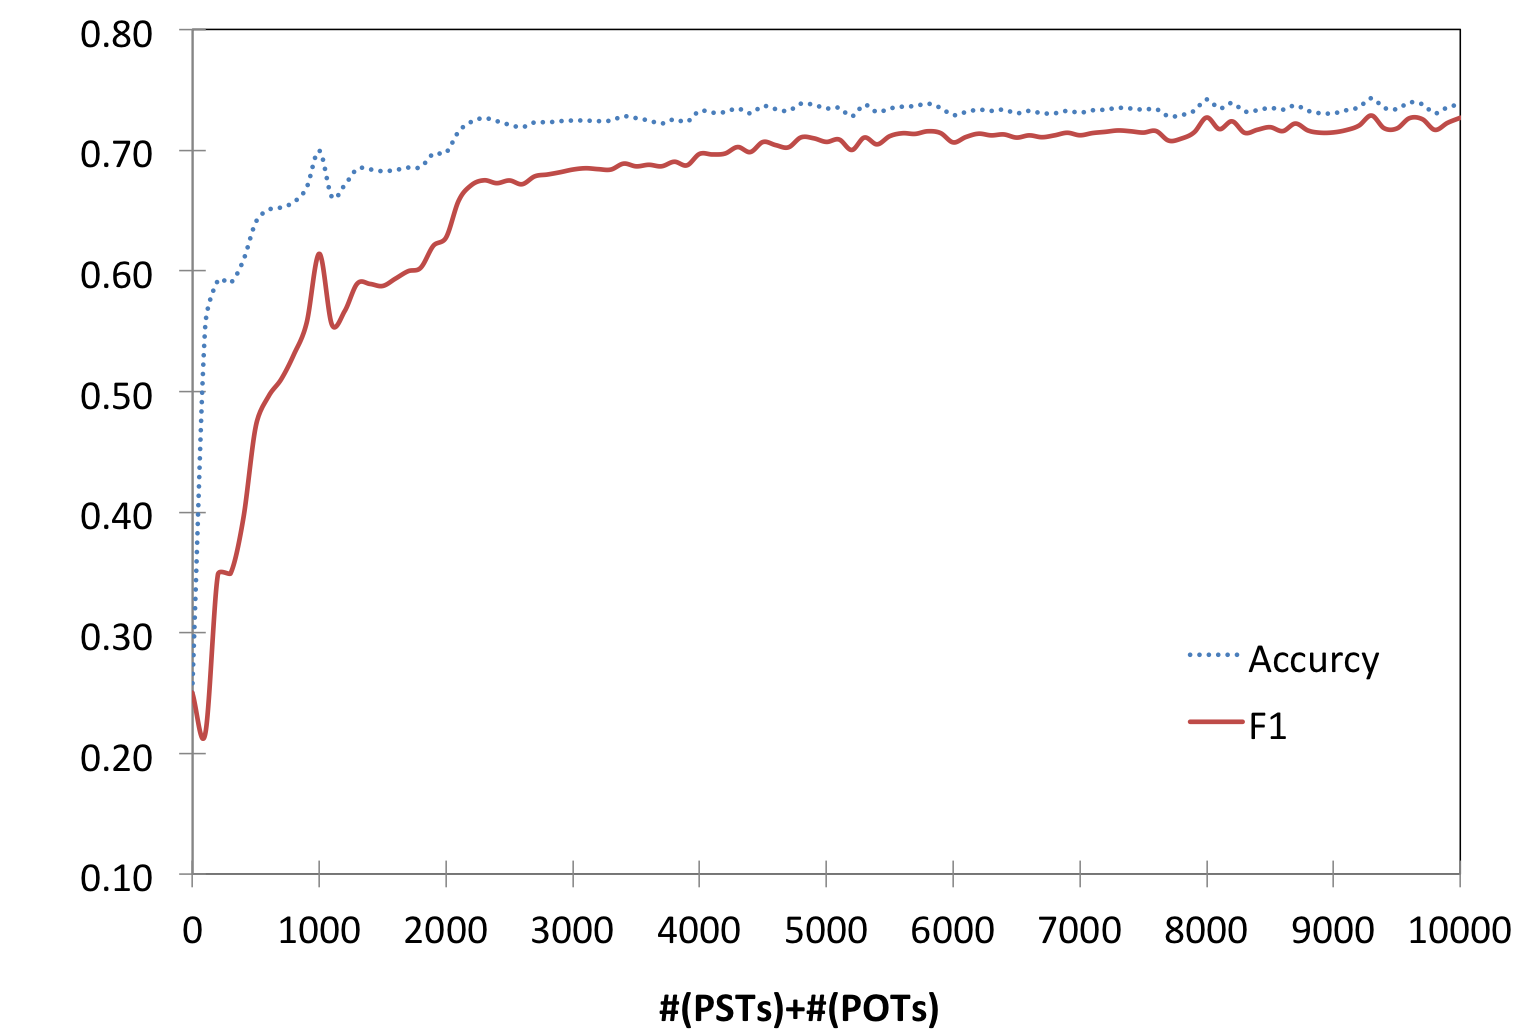
\includegraphics[height=250pt]{Sub_classify.png}
\caption{基于观点化特征的Twitter观点分类实验结果}
\label{Sub_classify}
\end{figure}

\subsubsection{基于观点化特征的Twitter观点分类实验结果}
\label{STC}
我们也对tweet观点化评价函数Opinion\_{avg}(d)能否作为主观化tweet的分类器感兴趣(见~\ref{form})。我们利用1000个手工标注的主观化tweet和1000个客观化tweet作为测试集。我们将Opinion\_{avg}(d)得分大于0的tweet视为主观化tweet,小于或等于0的tweet视为客观化tweet。正确率(Accuracy)和F1值作为分类器的评价指标。图~\ref{Sub_classify}给出了实验结果。我们发现当选取大约2200个PST和POT~tweet时,正确率与F1值趋于稳定,分别是0.72和0.67,再选取更多的PST和POT对于分类结果没有显著提高。这说明评价函数Opinion\_{avg}(d)对于tweet的主观化分类是有效的。


\subsubsection{最佳Twitter观点检索系统实验结果}
\label{AFE}

最后我们将所有在前面的实验中能够帮助Twitter观点检索的特征都加入到基准系统中形成新的检索模型。这些特征包括:BM25(或VSM)、链接(URL)、提及(Mention)、发布数目(Statuses)、粉丝数目(Followers)、Q\_D。表~\ref{bestBM25}和表~\ref{bestVSM}给出了Twitter观点检索最好的模型BM25\_Best和VSM\_Best在Twitter观点检索数据集上最好的实验结果,MAP值分别比系统BM25和VSM提高56.82\%和33.75\%。

另外,我们还将表~\ref{Features_Sum}中的所有特征整合到一个排序学习模型当中\footnote{这里我们只使用Q\_D评价一个tweet的观点化程度,因为它在前面的实验中对tweet的观点化评估效果最好。}。这里的两个排序模型分别称为BM25\_All和VSM\_All。表~\ref{bestBM25}和表~\ref{bestVSM}给出了这两个模型的排序结果,它们的排序能力稍微弱于BM25\_Best和VSM\_Best系统,但没有显著性差异。

以上结果表明,对于Twitter中的观点检索来说,仅仅使用特征BM25(或VSM)、链接(URL)、提及(Mention)、发布数目(Statuses)、粉丝数目(Followers)、Q\_D就能达到最佳效果。

\begin{table}
 \caption{基于全部与最佳特征的Twitter 观点检索系统实验结果(BM25)}
\label{bestBM25}
 \centering
 \begin{tabular}{|l l|}
 \hline
 & MAP \\
 \hline
BM25 & 0.2831\\
BM25\_Best & 0.4181$^\blacktriangle$\\
BM25\_All & 0.4128$^\blacktriangle$\\
 \hline
 \end{tabular}
      \begin{tablenotes}
        \footnotesize
\item $^\triangle$ 和$^\blacktriangle$分别表示排序结果显著高于BM25观点检索系统(p $<$ 0.05和p $<$ 0.01)。
\end{tablenotes}
\end{table}

\begin{table}
 \caption{基于全部与最佳特征的Twitter 观点检索系统实验结果(VSM)}
\label{bestVSM}
 \centering
 \begin{tabular}{|l l|}
 \hline
 & MAP \\
 \hline
VSM & 0.2812\\
VSM\_Best & 0.3761$^\blacktriangle$\\
VSM\_All & 0.3721$^\blacktriangle$\\
 \hline
 \end{tabular}
      \begin{tablenotes}
        \footnotesize
\item $^\triangle$ 和$^\blacktriangle$分别表示排序结果显著高于VSM观点检索系统(p $<$ 0.05和p $<$ 0.01)。
\end{tablenotes}
\end{table}

\subsection{Twitter观点检索实验数据偏置分析}
\label{TwitterBias}
因为目前还没有关于Twitter观点检索的数据,所以我们构造并标注了自己的数据集。但是仅仅使用BM25算法对每个查询词所对应的tweet进行排序,然后收集前100个tweet进行相关判定可能造成其它研究算法无法在这个数据集上实验验证。另外,用BM25算法收集的数据集可能由于该算法本身的问题造成选取数据的偏置。基本上由BM25算法选取的部分标记是否相关的文档去验证其它算法,有效性往往都无法很好的验证,这是因为所有排名100以外的未进行相关性判定的tweet都当做了不相关tweet,这也是TREC使用2个以上的检索算法返回结果形成“池”(Pool),且每个算法返回1000个或更多排序靠前文档进行数据相关性判定的原因。基于以上分析,我们利用了TREC2011年的Twitter信息检索任务的数据和其相关判定的结果来评价我们Twitter观点检索系统的有效性\footnote{下载地址:\url{http://trec.nist.gov/data/tweets/}}。

 TREC2011年的Twitter数据由1600万个tweet构成,这个数据从2011年两个星期的所有tweet数据中采样得到\upcite{ounis2011overview}。总共有59个来自世界各地的研究组织参加了Twitter信息检索任务的评测,并且提交了他们自身排序算法所得到的tweet排序结果。在TREC2011的Twitter信息检索数据集中总共包含49个话题(查询词)。每个研究组织被要求针对话题从1600万个tweet中检索30个tweet进行评价。最后返回结果所形成的tweet“池”有50324个tweet,其中2965个tweet被判定成话题相关tweet\footnote{下载地址:\url{http://trec.nist.gov/data/microblog/11/microblog11-qrels}}。但是,这些被判定为话题相关的tweet仅仅适合评价Twitter信息检索算法的有效性,而我们的目的是在Twitter中进行观点检索。因此,我们重新再手工标注了部分 TREC2011年的Twitter数据,判定哪个是话题相关且包含观点的tweet。我们利用Metzler等人提交的Twitter信息检索返回的结果重新标记(他们提交数据的ID是isiFDL)\upcite{metzler2011usc},选择Metzler等人提交的tweet是因为他们所提交的tweet返回结果是目前 TREC2011年的Twitter信息检索任务最好的结果\upcite{ounis2011overview},它包含了最多的话题相关的tweet。最后,我们重新标注的数据集中有98个话题相关且包含观点的tweet。

我们的方法是对Twitter中的数据进行观点检索,我们利用重新标注的TREC2011年的Twitter数据进行Twitter观点检索的实验验证,验证的方法是利用我们的系统对新标注的TREC数据进行重排序。我们将Metzler等人提出的Twitter信息检索系统作为基准系统\upcite{metzler2011usc},称为isiFDL。而我们利用链接(URL),提及(Mention),发布数目(Statuses),粉丝数目(Followers),Q\_D特征构造的系统称为{isiFDL\_Best,这里强调的是我们用算法isiFDL对tweet的话题相关性得分替换我们原先使用的BM25算法。我们同样使用5次交叉验证实验验证算法的有效性。表~\ref{trec}给出了实验结果。我们可以看到isiFDL\_Best系统对与Twitter观点检索的排序效果显著优于isiFDL系统。这说明我们的观点检索系统在重新标注的TREC2011Twitter数据上依然有效。

显然,虽然重新标注的数据最大限度地减小了话题相关的偏置问题,但是依然没有解决在观点化相关上的偏置问题。我们也不可能像TREC的方式一样组织多个研究机构提交Twitter观点检索的数据构造Twitter观点检索的标准数据。未来如果有像TREC一样的方式构造的Twitter观点检索数据,我们将再进一步验证我们方法的有效性。

\begin{table}
 \caption{ 观点检索系统在TREC Tweets201数据上的实验结果}
 \label{trec}
 \centering
 \begin{tabular}{|l l|}
 \hline
 & MAP \\
 \hline
isiFDL &0.1639\\
isiFDL\_Best&0.2181$^\triangle$\\
 \hline
 \end{tabular}
 \begin{tablenotes}
        \footnotesize
\item $^\triangle$ 和$^\blacktriangle$分别表示排序结果显著高于isiFDL观点检索系统(p $<$ 0.05和p $<$ 0.01)。
\end{tablenotes}
\end{table}

\section{小结}
据我们所知,我们是第一个提出如何在Twitter中进行观点检索的研究机构。我们的方法是利用社交媒体信息与tweet的观点化信息帮助检索。实验结果表明当检索模型中考虑链接(URL)、提及(Mention)、发布数目(statues)、粉丝数目(statues)、tweet文本的观点化程度等特征时,可以帮助提高Twitter观点检索效果。

另外,我们还提出了一种利用社交媒体信息和tweet文本结构化信息帮助生成近似主观化tweet(PST)和近似客观化tweet(POT)的方法,以此提高评估tweet观点化的程度,实验发现将其引入观点检索中可以替代传统手工标注数据的方法,且考虑话题相关因素构造PST和POT时,效果更好。
